\section{Data association}

When solving the \gls{SLAM} problem, an important issue is how the measurements are associated to the right landmark. This is relatively easy when you do feature-based \gls{SLAM}, e.g. when you use a visual slam system like ORB-SLAM \cite{ORBSLAM}. This is because the measurement itself has a direct way of being compared with other features for how alike they are, and a single point in space is usually pretty distinct. 

This is however not the case with the detection systems employed on Revolves race car. Since the cones are very similar, a feature extracting algorithm was not thought to work, and all the detection systems only give out a position in the plane, with the camera system outputting a cone color as well. This means the SLAM system needs to be able to keep track of which measurements belong to the same landmark. 

The problem of associating measurements to landmarks is what the SLAM literature refers to as the data association problem.

\subsubsection{Previous work}

Most of the work done on data association is for data association applied to object tracking, typically using a radar\cite{RadarTracking}, but also more recently to track visually\cite{VisualTracking}. Data association used for tracking implies finding out which of the tracked objects correspond to new measurements, where typically the measurements are all made from a stationary vantage point, while the objects are moving around. This means one must predict where the objects are going to be and try to match all observed objects with objects that are being tracked. 

Data association applied to \gls{SLAM} have gotten more common in the recent years. It is an almost opposite problem to the tracking problem, as the observer is the one moving around, while the landmarks are standing still. While a lot of the work done on tracking focuses on a single or a handful of objects to track, when solving the \gls{SLAM} problem one by definition wants to be able to handle a large amount of landmarks. This is because the output of the system is going to be the map, and the system needs to be able to handle all the landmarks that build up the map. The data association problem met in the two settings are however quite similar, and work done in one field therefore benefits the other. 

\subsection{Nearest Neighbour}

When talking about the data association problem and its solutions it is essential to keep in mind at all times what application is being discussed. In many of the earlier cases the tracking problem is simply matching measurements with one object, in which case a nearest neighbour matching with the Malahanobis distance can work wonders\cite{ShalomTracking}. 

In this case it is assumed that one of the measurements is the object, and you are simply trying to know which one it most likely is. It's assumed that the objects movement can be approximated as

\begin{equation}
    p_{next} = Ap_{prev} + w_{model}
\end{equation}

The objects location is then measured with a measurement model

\begin{equation}
    p_{meas} = Hp_{true} + w_{meas}
\end{equation}
 
Here A is the linearized dynamic model for how the object moves, H is the linearized measurement function and $w_{model}$ and $w_{meas}$ are additive zero-mean white noise for the model and measurement, respectively. It then uses a Kalman filter step to propagate the expected position and covariance of the object using the previous position, the dynamic model of the object and a covariance for both the previous position and the dynamic model. This then gives the new estimated position of the object and it's covariance. Using the estimated and measured positions and covariances, the nearest neighbour is then found using the Mahalanobis distance\cite{MahalanobisTracking}:

\begin{equation}
    d^2_{Mahala} = (p_{est} - p_{meas})^T(\Sigma_{est} - \Sigma_{meas})^{-1}(p_{est} - p_{meas})
\end{equation}

The Mahalanobis distance can be seen as a scaled euclidean distance, where the reference frame is rotated to match the principal axes of the underlying Gaussian distribution and the axes are scaled to the variance along the principal axes of this distribution. This means that a unit length in the euclidean sense is larger if it is in a direction where the variance is small and vice versa. The height curves of the Gaussian and its principal axes are illustrated in figure \ref{Fig:GaussianPrincipalAxes}. 

\begin{figure}
    \centering
    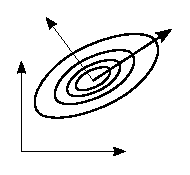
\includegraphics[width=0.5\linewidth]{0_Images/3_Theory/GaussianPrincipalAxis.eps}
    \captionof{figure}{Height curves of a Gaussian distribution, with its principal axes.}
    \label{Fig:GaussianPrincipalAxes}
\end{figure}

\subsection{Probabilistic Data Association Filter}

The problem with the above method is that, even when the dynamics of the object and the measurement function are in fact linear and known perfectly, there is a non-zero probability that the measurement used to update the object is the wrong measurement, in which case track might be lost. A more sophisticated approach that tracks one target in the presence of false alarms and low probability of detection at each time step, is \gls{PDA}\cite{BarShalomPDA}. Instead of assigning one measurement to the object at each instant, it uses all the validated measurements to update the object, weighting each measurement with the probability that they actually are from the object.  

Much like the nearest neighbour association, it assumes a known linear state transition with additive white noise

\begin{equation}
    x_{k+1} = F_kx_k + w_k, k=0,1,2..
\end{equation}

where $F_k$ is known, $w_k$ has zero mean and a known variance of 

\begin{equation}
    E(w_kw_j') = Q_k\delta_{kj}
\end{equation}

The initial state is assumed normally distributed with mean $\hat{x}_{0|0}$ and covariance $P_{0|0}$, independent of $w_k$. Similarly it is assumed a known linear measurement function with additive white noise

\begin{equation}
    z_k = H_kx_k + y_k, k = 1,2,..
\end{equation}

where $H_k$ is known and $y_k$ is the measurement noise with zero mean known variance 

\begin{equation}
    E(v_kv_j') = R_k\delta_{kj}
\end{equation}



Furthermore it assumes a validation method that guarantees that the correct measurement will be kept with a certain probability. It also assumes that the false positives are spatially uniform and independent. The number of false positives at each time instant is not known exactly.   

The validation method used is to reject measurement $i$ if it doesn't pass the following test

\begin{equation}
    \nu_{k,i}'S_k^{-1}\nu_{k,i} \leq \gamma
\end{equation}

where 

\begin{equation}
    S_k = H_kP_{k|k-1}H'_k+R_k
\end{equation}

and $\nu_{k,i} = z_{k,i} - \hat{z}_{k|k-1}$ is the difference between measurement $z_{k,i}$ and the predicted object position $\hat{z}_{k|k-1}$ at time step $k$. $\gamma$ is the validation gate threshold. This assures that the correct measurement has a non-zero probability of being kept. 

The linearity assumptions added above is later removed and accounted for by increasing the covariances on the state transition and measurement. Each validated measurement is used to update the object position, and it is shown on a highly nonlinear simulation problem that the resulting track is better than both the nearest neighbour filter and a track splitting filter, where each new measurement spawns a new filter. The latter is exponential in the number of false positives, so it is very unfeasible in many situations. 

\subsection{Joint Probabilistic Data Association}

To handle the more useful case of having more than one object to track in the presence of uniform Poisson clutter, the \gls{JPDA} method was developed\cite{JPDA}. It assumes several objects, uniformly distributed clutter in the neighbourhood of the objects and low probabilities of detecting the targets at each time step. When the targets are far enough away that none of the same measurements are possible to associate to both, the algorithm is like running several \glspl{PDA} in parallel. However, when measurements are possible to associate to more than one target, \gls{JPDA} takes this into account. 

This leads to good tracking, but at the cost of a much higher computational cost, especially when there are many targets. In addition it assumes the number of targets are known, and has no logic to initialise and terminate possible tracks. This is dealt with in \cite{Multitrack}. In \cite{JPDARev} the $M$ best possible permutations of measurement to target matches are found using \gls{LP}. This leads to a massive reduction in runtime compared with the pure \gls{JPDA}, while retaining most of the performance. Like with the \gls{JPDA} it does however not handle initialising and terminating tracks. This is assumed to be done by an operator.

\subsection{Joint Maximum Likelihood}

A data association method developed specifically for \gls{SLAM} is the \gls{JMH}\cite{JMH}. It aims to solve the problem of uniquely associating a batch of measurements of landmarks to existing landmarks. \gls{JMH} frames the tracking problem as the problem of finding the set, $E_k = \{ e_1, e_2, ... , e_m\} $, of associations, where each element $e_n = \{i,j\}$ is a binary association between measurement $i$ and landmark $j$ that maximises the products of likelihoods

\begin{equation}
    E_k = \argmax_{E_l} \prod_{\forall e_m \in E_l} f_{e_{i,j}}
\end{equation}

where 

\begin{equation}
    f_{i,j} = \frac{1}{(2\pi)^{n/2}} exp(-\frac{1}{2}\nu_{i,j}^T\delta_j^{-1}\nu_{i,j})
\end{equation}

To avoid overflow this is transformed into maximising the sum of the log-likelihoods instead.

\begin{equation}
    E_k = \argmax_{E_l} \sum_{\forall e_m \in E_l} ln(f_{em})
\end{equation}

which is then the same as finding the $E_l$ that minimises the sum of the Malahanobis distances

\begin{equation}
    E_k = \argmin_{E_l} \sum_{\forall e_m \in E_l} N_{e_m}
\end{equation}

where 

\begin{equation}
    N_{e_m} = \nu_{i,j}^TS_j^{-1}\nu_{i,j} 
\end{equation}

\subsection{Joint Compatibility}

Doing almost the same as the \gls{JMH}, but instead of minimising the normalised distances, one aims to find a set that gives as many measurement-landmark associations that satisfy the compatibility test

\begin{equation}
    \nu_{i,j}^TS_j^{-1}\nu_{i,j} \leq \gamma_n
\end{equation}

as possible. Here $\gamma_n$ is usually taken to be around $0.95$, i.e. that it is $\SI{95}{\percent}$ probable that measurement $i$ came from landmark $j$. This problem is known as Joint Compatibility, and one solution is found in \cite{Bailey}
